\section{Statement for Plan of Work}
For the remaining 8 weeks, development of CapitalGames will be divided into two major deliverables. The first deliverable will be a beta release featuring all functionality outlined in previous reports. This first deliverable is expected to be completed by the last week in March. Following the completion of this milestone, CapitalGames will be offered to a private alpha community to gather valuable feedback and do at-scale bug testing. We feel that this development pattern, closely resembling the agile development methodology, will allow us to build the most stable and effective product in the remaining time of this project.  \\

\section{First Deliverable (Demo 1)}
\subsection{Logic Implementation}
The logic of the first deliverable is further divided into subcomponents which are the primary pillars of CapitalGames. \\
\subsubsection{1. Routing Scheme}
The first component is finalizing and configuring the routing scheme for this system since the particular framework used for implementation has a fairly strict one-to-one association between object organization and routing. To clarify, the routing scheme is the mapping of publically accessible resources (URI’s) to internal resources. The routing component will be finished by beginning of the week of March 17th. \\
\subsubsection{2. Users}
Since the site centers around the user, by both educating about personal finance and entertaining in a fantasy trading world, the logical next component to implement is the User component. This incorporates the development of the user/related models as well as authentication and management systems. This component is scheduled for completion during the second half of the week of March 17th. \\
\subsubsection{3. Leagues}
The Leagues component holds most of the business logic of CapitalGames and therefore its important that development on this component immediately follows the completion of the Users component. The Leagues component holds all the functionality concerning trading of stocks, league management and overall performance tracking. The projected deadline for this component is the beginning of the week of March 24th. \\ 
\subsubsection{4. Portfolios}
The Portfolio is logically developed after the League component is finished, as its functionality is only valid in the context of a league. The Portfolio component deals with representing a user and his/her performance in the context of a league. This means it stores the personal performance as well as activity that a user does within any particular league. All transactions of a user are also stored for various purposes such as conducting statistical analysis on the site as a whole. The background process subsystem is also developed during this stage. The Portfolios component is scheduled for completion by the end of the week of March 24th. \\

\subsection{User Experience}
The development of the user interface is handled independently from the implementation of the backend logic. Once both subsystems near completion, the integration process will begin. The projected timeline for the user interface is presented below and closely lines up with the logic timeline presented above: \\
\subsubsection{1. View Structure Finalization}
Similar to the routing scheme, the view organization in this MVC based framework requires careful planning of how views will be implemented. Therefore, the first step in user interface implementation is finalizing the structure of views in the CapitalGames system. This will be done during a hacking event coordinated by our group on March 18th. \\
\subsubsection{2. Customizing “Dashboard Admin” theme}
The next step in the user interface implementation is the customization of a very featureful them called “Dashboard Admin”. During this stage the theme is molded into the view structure finalized in the previous step. In other words, certain elements in each theme are split into appropriate views/sub-views. This is, however, not the stage at which minute design tweaks are done. These fine-grain modifications are saved for the end in order not to prolong this stage. The customization process is scheduled for completion by the end of the week of March 18th. \\
\subsubsection{3. Implement Design Tweaks}
The subsequent step is likely the most artistic one. It involves tweaking the stock theme and making it more characteristic of the CapitalGames brand. From past experience, this is a stage that can easily become very dragged out so in order to stick to a safe schedule, a strict deadline of end of March is set for this task. \\
\subsubsection{4. Visualization \& AJAX Integration}
Since a major component of this system is the visualization of trends and trading data, the integration of the HighCharts visualization library is considered a separate stage. This is closely coupled with the asynchronous communication between the UI and backend, which will improve the user experience and make the system more responsive. These two subcomponents will be implemented by end of March as well.\\

\section{Second Deliverable (Demo 2)}
For both the logic and user experience sides of the system, the following timeline of events applies. This timeline is slightly more malleable as feedback quality/quantity can’t be accurately projected. \\
\subsubsection{1. Responding to feedback}
Since the development team of 6 people can’t possibly figure out every way to make the best possible CapitalGames, a week and a half long period is devoted to responding to user feedback. This will include both suggestions for improvements as well as bugs identified by alpha testers. This period is scheduled to occur middle of the last week of March to the end of the first week of April. \\
\subsubsection{2. Respond to bug fixes, finalize integration}
A full two weeks are dedicated to responding to other technical issues identified by our team. This includes everything from functional errors to performance issues. This period is also allocated to finalizing the integration of the UI and logic systems as this can take an unexpectedly long amount of time. \\

\section{Breakdown of Responsibilities}
\subsubsection{Jeff Rabinowitz}
Jeff will be leading the routing scheme and unit testing aspects of CapitalGames. This will include finalizing the routing configuration and managing unit testing of modules built by other members. He has the ability to delegate unit-testing responsibilities to other members. \\
\subsubsection{Eric Cuiffo}
Eric will be leading the user interface development. To this extent, he will be responsible for ensuring that progress of UI development stays on track with our schedule. While he will personally implement a lot of the front end, Dario and Nick will also play key roles in front end development. \\
\subsubsection{Nick Palumbo}
Nick’s primary responsibilities will include model design and implementation across multiple modules. This means he will be closely working with the DB and ensuring that the states of user, league, and portfolio models are consistently represented throughout the system. He will also be leading integration testing with Dario and be helping front-end development where necessary. \\
\subsubsection{Jeff Adler}
Jeff will be leading the background process system that is used for both processing transactions and performing performance calculations. He will be implementing a lot of this system with the help of Dario. In addition, he will be responsible for the configuration and management of our back-end server.\\
\subsubsection{Val Red}
Val will be leading the finance system, which communicates directly with the Yahoo Finance API and translates it into models relevant to our system. His responsibilities will therefore span across both the leagues and portfolio components. Due to his prior experience with the MySQL engine, he will likely aid the model design and DB interactions tasks being lead by Nick. \\
\subsubsection{Dario Rethage}
Dario will lead system integration throughout the development process due to his prior experience working with distributed architectures. This includes UI to backend integration as well as integrating various third party frameworks such as the Resque library or the HighCharts library. After the first deliverable is complete, he will focus more on integration testing with Nick. Dario will also play an active role in UI development and a supportive role in the background process subsystem. \\

\hfil\eject \pdfpagewidth=8.5in \pdfpageheight=16in
\begin{figure}
\section{Gantt Chart of Projected Milestones} 
Best viewed at 100\% or greater:    
\centering
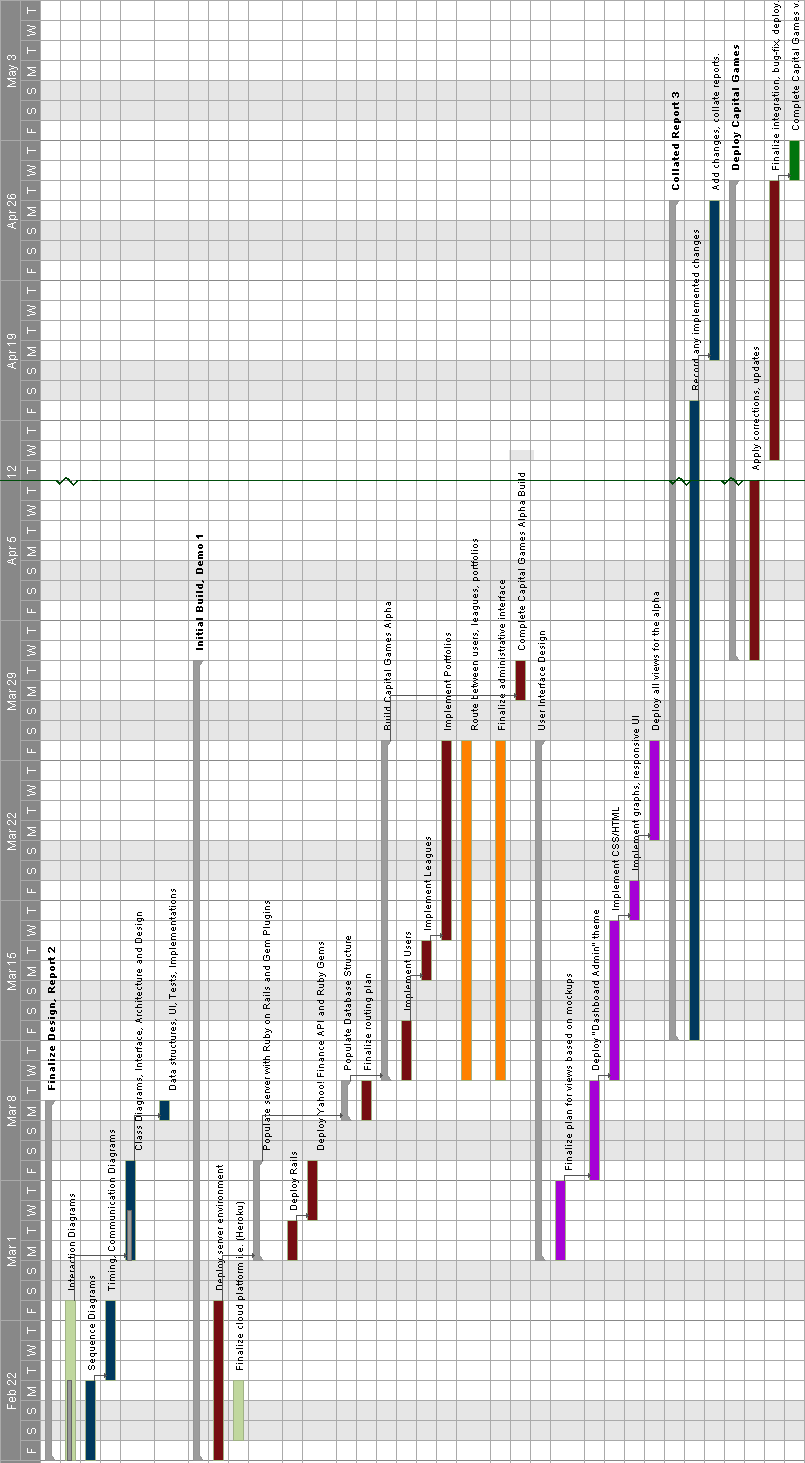
\includegraphics[width=6.5in]{./img/gantt.png}
\caption{This gantt chart projects how we will concurrently work on
the project. All blue items are report-related, red and orange relate
to the core project development and purple illustrates UI milestones.}
\end{figure}
